\newpage
\section{Mô hình hồi quy tuyến tính kết hợp với các phương pháp PCA(Principal Component Analysis)}

\paragraph{}{PCA (Principal Component Analysis) giúp giảm chiều dữ liệu bằng cách tìm ra các \textbf{thành phần chính (Principal Components - PCs)} mà vẫn giữ được nhiều thông tin nhất. Trong tập dữ liệu này, ta có nhiều biến liên quan đến nhau (tương quan cao), nên việc dùng PCA giúp:}

\begin{itemize}
    \item \textbf{Giảm đa cộng tuyến} (nhiều biến có tương quan cao sẽ gây khó khăn cho mô hình dự đoán).
    \item \textbf{Tăng hiệu suất tính toán} (mô hình không cần xử lý quá nhiều biến).
    \item \textbf{Loại bỏ nhiễu} và \textbf{giữ lại thông tin quan trọng} nhất.
\end{itemize}

\subsection{Phân tích tương quan và chọn nhóm biến}
\label{subsec:correlation}

\begin{figure}[H] 
    \centering
    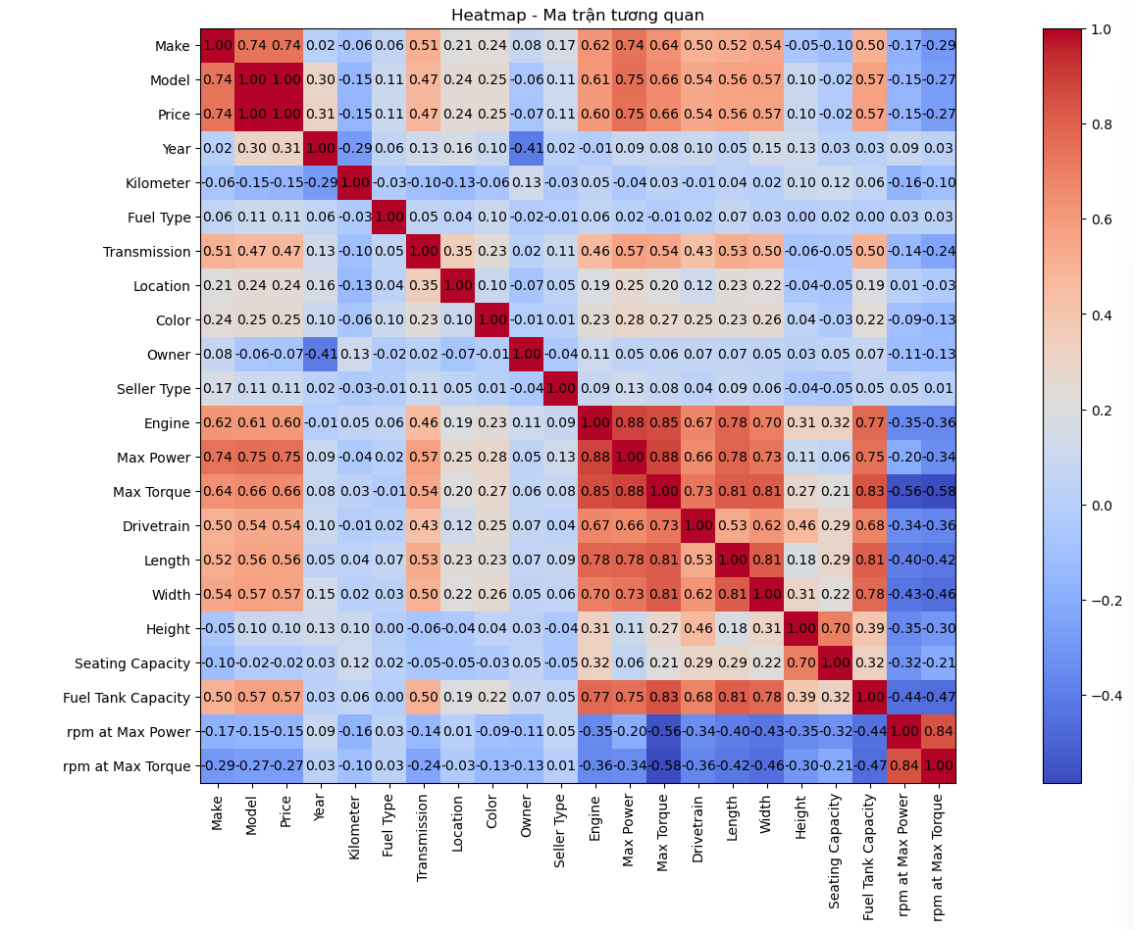
\includegraphics[width=1\textwidth]{img/heatmapPCA.png} 
    \caption{Ma trận tương quan giữa các biến.}
    \label{fig:correlation_matrix}
\end{figure}

\paragraph{}{Phân tích ma trận tương quan cho thấy các nhóm biến có mối liên hệ chặt chẽ:}
\begin{itemize}
    \item \textbf{Nhóm kích thước xe} (\texttt{Seating Capacity}, \texttt{Length}, \texttt{Height}, \texttt{Width}, \texttt{Fuel Tank Capacity}) có mối tương quan cao, đặc biệt giữa \texttt{Length} - \texttt{Width} (0.81), \texttt{Height} - \texttt{Seating Capacity} (0.7) và \texttt{Fuel Tank Capacity} - \texttt{Width} (0.78), cho thấy khả năng giảm chiều dữ liệu.
    \item \textbf{Nhóm công suất động cơ} (\texttt{Engine}, \texttt{Max Power}, \texttt{Max Torque}, \texttt{Drivetrain}) có quan hệ chặt chẽ, với \texttt{Engine} - \texttt{Max Power} (0.88) và \texttt{Max Power} - \texttt{Max Torque} (0.88). \texttt{Drivetrain} - \texttt{Max Torque} (0.72) cho thấy khả năng giảm chiều dữ liệu.
    \item \textbf{Nhóm vòng tua động cơ} (\texttt{rpm at Max Power}, \texttt{rpm at Max Torque}) có tương quan 0.84, thể hiện mối quan hệ tuyến tính mạnh, phù hợp để giảm số chiều dữ liệu.
\end{itemize}

\subsection{Áp dụng phương pháp PCA}
\label{label: PCA}
\label{subsec:apply_pca}

\paragraph{}{PCA được áp dụng trên ba nhóm biến có tương quan cao nhằm giảm chiều dữ liệu mà vẫn bảo toàn thông tin quan trọng. Quá trình thực hiện gồm các bước:}

\begin{enumerate}
    \item \textbf{Áp dụng PCA trên tập train}:
    \begin{itemize}
        \item Áp dụng phương pháp PCA (xem các bước thực hiện ở \ref{label: pca})
        \item Kết quả thu được ba đặc trưng mới: \texttt{PCA\_hs}, \texttt{PCA\_cs}, \texttt{PCA\_kt}.
        \item Các cột ban đầu được loại bỏ khỏi tập dữ liệu.
    \end{itemize}
    \item \textbf{Áp dụng PCA trên tập validation}:
    \begin{itemize}
        \item Sử dụng giá trị trung bình và vector thành phần chính từ tập train để biến đổi dữ liệu validation, đảm bảo nhất quán.
        \item Thay thế các biến gốc bằng các đặc trưng PCA tương ứng.
    \end{itemize}
\end{enumerate}

\paragraph{}{Sau khi áp dụng \textbf{PCA}, ta thu được các 13 đặc trưng gồm \texttt{PCA\_hs}, \texttt{PCA\_cs}, \texttt{PCA\_kt}, cùng với các đặc trưng ban đầu như \texttt{Make}, \texttt{Model}, \texttt{Year}, \texttt{Kilometer}, \texttt{Fuel Type}, \texttt{Transmission}, \texttt{Location}, \texttt{Color}, \texttt{Owner}, \texttt{Seller Type} dùng dể dự đoán giá xe $Price$}

\label{sec:training_evaluation}

\subsection{Chuẩn hóa dữ liệu và chia tập dữ liệu để huấn luyện}
\label{subsec:preprocessing}

\begin{itemize}
    \item \textbf{Chuẩn hóa dữ liệu} bằng phương pháp Z-score (xem \ref{label:standart scaler}). Việc này giúp đưa dữ liệu về cùng một thang đo, giảm ảnh hưởng của đơn vị đo khác nhau và cải thiện tốc độ hội tụ của thuật toán tối ưu (xem \ref{label:toc do hoi tu}).
    % (chứng minh phần Tốc độ Gradient decent khi đưa về ) % -> Có thể thêm tham chiếu đến phụ lục hoặc phần khác nếu có
    \item \textbf{Chia tập dữ liệu}:
    \begin{itemize}
        \item $X_{\text{train\_v2}}$, $X_{\text{val\_v2}}$: Đặc trưng đầu vào (sau chuẩn hóa và PCA).
        \item $y_{\text{train\_v2}}$, $y_{\text{val\_v2}}$: Biến mục tiêu (\texttt{Price}).
    \end{itemize}
\end{itemize}

\subsection{Xây dựng mô hình}
\label{subsec:model_building}
\subsubsection{Phương pháp xây dựng}
\paragraph{}{Mô hình hồi quy tuyến tính đa biến (Multiple Linear Regression) (xem ở \ref{label:lr}) được xây dựng để dự đoán giá xe dựa trên các đặc trưng đã xử lý (bao gồm các thành phần từ PCA và các biến khác).}

\subsubsection{Huấn luyện mô hình}


\paragraph{}{\textbf{Các siêu tham số:}}
\begin{itemize}
    \item Learning rate: 0.001
    \item Số epoch: 200
    \item Batch size: 32
\end{itemize}

\paragraph{}{\textbf{Triển khai:}}
\begin{itemize}
    \item Dữ liệu huấn luyện được xáo trộn trước mỗi epoch để giảm thiểu phương sai trong quá trình cập nhật trọng số.
    \item Batch Gradient Descent được sử dụng để cập nhật trọng số mô hình.
    \item Lưu lại bộ trọng số tốt nhất trong quá trình huấn luyện.
\end{itemize}

\paragraph{}{\textbf{Quá trình huấn luyện:}}

\begin{figure}[H]
    \centering
    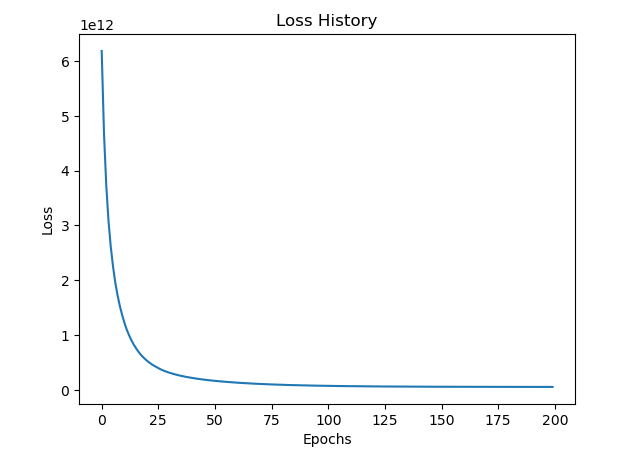
\includegraphics[width=0.7\textwidth]{img/lossPCA.png} % Điều chỉnh width nếu cần
    \caption{Biểu đồ Loss qua các Epoch.}
    \label{fig:loss_plot}
\end{figure}

\begin{itemize}
    \item Biểu đồ cho thấy giá trị hàm mất mát (Loss) giảm dần theo số epoch, chứng tỏ mô hình đang học được các mẫu từ dữ liệu huấn luyện.
    \item Ban đầu, loss rất lớn (khoảng $1369526006662$), nhưng sau 200 epoch, nó giảm xuống đáng kể còn khoảng $552622539599.0718$.
    \item Mô hình đạt được giá trị loss tối ưu (trên tập huấn luyện là $552622539599.0718$)
\end{itemize}
\subsubsection{Công thức hồi quy}
\[
\begin{aligned}
Price = 1715141.18 &+ 57577.71 x_1 + 2332775.74 x_2 + 39443.65 x_3 \\
              &- 7834.82 x_4 + 1770.64 x_5 - 11278.79 x_6 \\
              &- 3295.49 x_7 - 4708.11 x_8 - 18789.88 x_9 \\
              &+ 7566.50 x_{10} + 11094.97 x_{11} - 7151.10 x_{12} \\
              &- 4041.87 x_{13}
\end{aligned}
\]
\paragraph{}{Trong đó:}
\begin{itemize}
    \item $Price$: Giá xe được dự đoán bởi mô hình
    \item $x_i$ với $i \in \{1, 2, \dots, 13\}$: Giá trị của các đặc trưng sau các quá trình xử lí dữ liệu và quá trình PCA (xem \ref{label: PCA})
\end{itemize}
\subsection{Đánh giá mô hình}

\begin{figure}[H]
    \centering
    \begin{subfigure}[b]{0.445\textwidth}
        \centering
        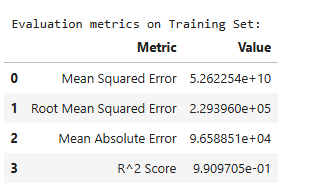
\includegraphics[width=\linewidth]{img/metrictrainPCA.png}
        \caption{Đánh giá trên tập huấn luyện}
        \label{fig:PCA-linear-train}
    \end{subfigure}
    \hfill
    \begin{subfigure}[b]{0.48\textwidth}
        \centering
        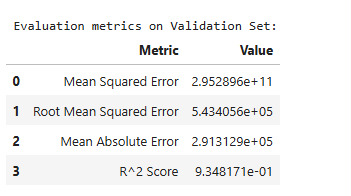
\includegraphics[width=\linewidth]{img/metricvalPCA.png}
        \caption{Đánh giá trên tập kiểm chứng}
        \label{fig:PCAlinear-valid}
    \end{subfigure}
    \caption{So sánh đánh giá mô hình trên tập huấn luyện và kiểm chứng} 
    \label{fig:PCA-linear-eval}
\end{figure}
\paragraph{}{
Trên tập huấn luyện, mô hình đạt MSE là \( 5.262254 \times 10^{10} \) và \( R^2 \) là \( 0.9910 \) (từ \( 9.909705e-01 \)), cho thấy mô hình đã học tốt giữa biến đầu vào biến đầu ra. Tuy nhiên, trên tập kiểm chứng, MSE tăng lên đáng kể thành \( 2.952896 \times 10^{11} \) và \( R^2 \) giảm xuống còn \( 0.9348 \) (từ \( 9.348171e-01 \)).

Mặc dù \( R^2 \) trên tập kiểm chứng vẫn khá cao, sự gia tăng đáng kể của các chỉ số lỗi (MSE tăng từ \( 5.26 \times 10^{10} \) lên \( 2.95 \times 10^{11} \)) cho thấy dấu hiệu của hiện tượng overfitting. Điều này cho thấy rằng mô hình đã học quá tốt trên bộ dữ liệu, làm giảm khả năng tổng quát hóa trên bộ dữ liệu mới.

Biểu đồ “Actual vs Predicted” minh họa sự so sánh giữa giá trị thực tế và giá trị dự đoán của mô hình (quan sát thấy trong hình \ref{fig:PCAactual-linear-eval}). Nhìn chung trên tập huấn luyện và kiểm chứng, các dữ liệu tập trung gần đường thẳng hồi quy cho thấy rằng mô hình dự đoán tương đối tốt xu hướng chung. Tuy nhiên, trên tập kiểm chứng, các điểm dữ liệu phân tán rộng xung quanh đường hồi quy (Có thể là kết quả của các giá trị ngoại lai hoặc những trường hợp mô hình dự đoán chưa chính xác).

Từ những nhận xét trên, ta thấy rằng mô hình hoạt động khá tốt với dữ liệu khi được áp dụng phương pháp PCA (Principal Component Analysis) và áp dụng phương pháp chuẩn hóa Z-score. Đúng với cơ sở lý thuyết toán học đã viết ở trên (\ref{label:toc do hoi tu}, \ref{label: pca}).
}


\begin{figure}[H]
    \centering
    \begin{subfigure}[b]{0.5131\textwidth}
        \centering
        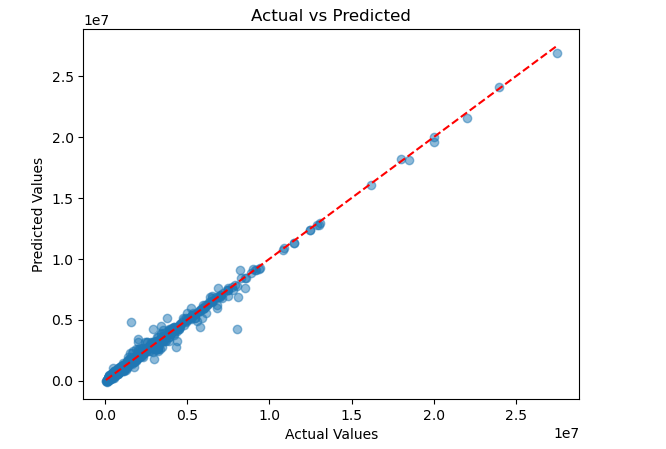
\includegraphics[width=\linewidth]{img/actualtrain.png}
        \caption{Đánh giá trên tập huấn luyện}
        \label{fig:PCAactual-linear-train}
    \end{subfigure}
    \hfill
    \begin{subfigure}[b]{0.465\textwidth}
        \centering
        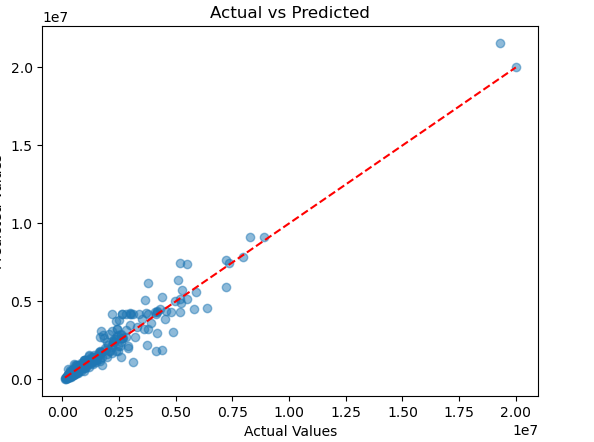
\includegraphics[width=\linewidth]{img/actualval.png}
        \caption{Đánh giá trên tập kiểm chứng}
        \label{fig:PCAactual-linear-valid}
    \end{subfigure}
    \caption{Đường thẳng hồi quy dự đoán so với thực tế, trên tập huấn luyện và kiểm chứng} 
    \label{fig:PCAactual-linear-eval}
\end{figure}

\pagebreak